\begin{figure*}[h]
  \centering
  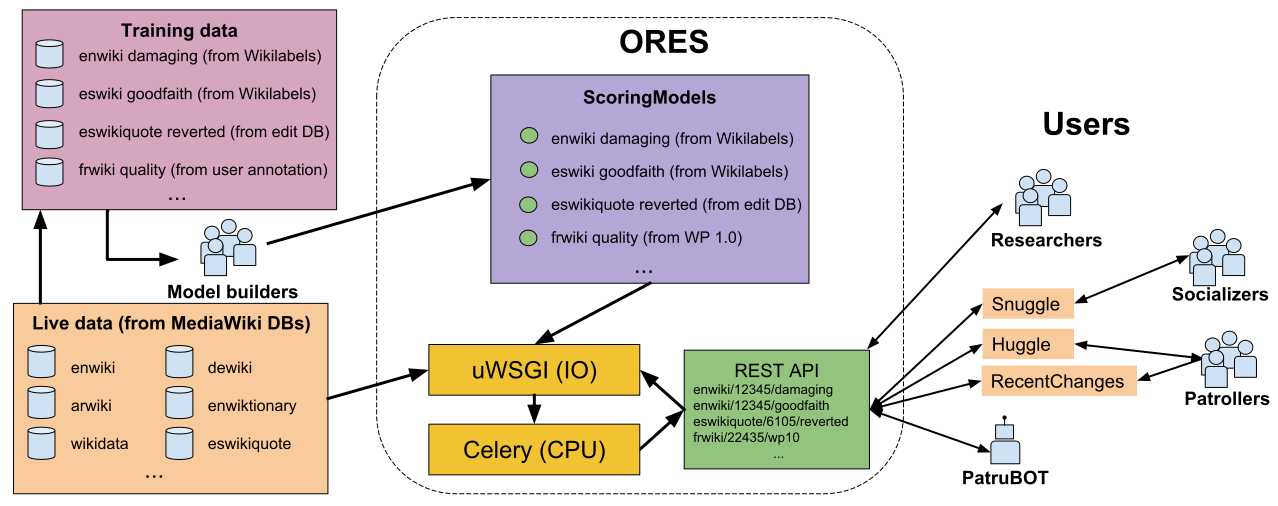
\includegraphics[width=.95\textwidth]{figures/ores_data_user_diagram}
  \caption{ORES conceptual overview.  Model builders design process for training ScoringModels from training data.  ORES hosts ScoringModels and makes them available to researchers and tool developers.}
  \label{fig:ores_data_user}
\end{figure*}

ORES has been iteratively engineered to meet the needs of Wikipedia editors and the tools that support their work (see section~\ref{sec:ores_system_engineering}). It is a machine learning as a service platform that enables Wikipedians and researchers to commission a new classifier, which are hosted by the Wikimedia Foundation for anyone to query. Figure  \ref{fig:ores_data_user} gives a conceptual overview, showing how ORES is a collection of machine classifier models and an web-based API, which connect to various sources of training data (to build the models) and live data (to apply the models). These models are designed and engineered by a varied set of model builders, some are external researchers and others are our own engineering team.  The models that ORES hosts are based on quite different sets of curated training data and have been engineered to support Wikipedian processes related to damage-detection, quality-assessment, and topic-routing. In general, the system is adaptable to a wide range of other models.

To make these models available for users, ORES implements a simple container service where the ``container,'' referred to as a \emph{ScoringModel}, represents a fully trained and tested prediction model.  All \emph{ScoringModels} contain metadata about when the model was train/tested and code for feature extraction.  All predictions take the form of a JSON document.  The ORES service provides access to ScoringModels via a RESTful HTTP interface and serves the predictions to users (see Figure~\ref{fig:english_wp10_prediction} for an example score request/response).  We chose this service structure because Wikimedian tool developers (our target audience) are familiar with this RESTful API/JSON workflow due to their common use of the MediaWiki API which employs a similar pattern.  While our target users may not have the expertise to build and maintain machine prediction models, they clearly have the expertise to make use this type of external API.

\subsection{Score documents}
\label{sec:appendix.score_documents}
The predictions made by ORES are human- and machine-readable.  In general, our classifiers will report a specific prediction along with a set of probability (likelihood) for each class.  By providing detailed information about a prediction, we allow users to re-purpose the prediction for their on use.  Consider the article quality (wp10) prediction output in Figure~\ref{fig:english_wp10_prediction}.

\begin{figure}[h!]
        \makebox{\hrulefill}{
        \small
        \begin{verbatim}
"wp10": {
  "score": {
    "prediction": "Start",
    "probability": {
      "FA": 0.00329313015, "GA": 0.0058529554,
      "B": 0.06062338048, "C": 0.01991363271,
      "Start": 0.754330134, "Stub": 0.1559867667
    }
  }
}
        \end{verbatim}
        \hrule
        \normalsize}
        \caption{A score document -- the result of \url{https://ores.wikimedia.org/v3/scores/enwiki/34234210/wp10}}
        \label{fig:english_wp10_prediction}
\end{figure}

A developer making use of a prediction like this may choose to present the raw prediction ``Start'' (one of the lower quality classes) to users or to implement some visualization of the probability distribution across predicted classed (75\% Start, 16\% Stub, etc.).  They might even choose to build an aggregate metric that weights the quality classes by their prediction weight (e.g. Ross's student support interface\cite{ross2016visualizing} or the \emph{weighted sum} metric from~\cite{halfaker2017interpolating}).

\subsection{Model information}
\label{sec:appendix.model_information}
In order to use a model effectively in practice, a user needs to know what to expect from model performance.  E.g. how often is it that when an edit is predicted to be ``damaging'' it actually is? (\emph{precision}) or what proportion of damaging edits should I expect will be caught by the model? (\emph{recall})  The target metric of an operational concern depends strongly on the intended use of the model.  Given that our goal with ORES is to allow people to experiment with the use and to appropriate prediction models in novel ways, we sought to build an general model information strategy.

\begin{figure}[htbp]
        \makebox{\hrulefill}{
        \small
        \begin{verbatim}
"damaging": {
  "type": "GradientBoosting",
  "version": "0.4.0",
  "environment": {"machine": "x86_64", ...},
  "params": {"center": true, "init": null,
             "label_weights": {"true": 10},
             "labels": [true, false],
             "learning_rate": 0.01,
             "min_samples_leaf": 1,
             ...},
  "statistics": {
    "counts": {
      "labels": {"false": 18702, "true": 743},
      "n": 19445,
      "predictions": {
        "false": {"false": 17989, "true": 713},
        "true": {"false": 331, "true": 412}}},
    "precision": {
      "labels": {"false": 0.984, "true": 0.34},
      "macro": 0.662, "micro": 0.962},
    "recall": {
      "labels": {"false": 0.962, "true": 0.555},
      "macro": 0.758, "micro": 0.948},
    "pr_auc": {
      "labels": {"false": 0.997, "true": 0.445},
      "macro": 0.721, "micro": 0.978},
    "roc_auc": {
      "labels": {"false": 0.923, "true": 0.923},
      "macro": 0.923, "micro": 0.923},
    ...
  }
}
        \end{verbatim}
        \hrule
        \normalsize}
        \caption{Model information for an English Wikipedia damage detection model -- the result of \url{https://ores.wikimedia.org/v3/scores/enwiki/?model_info&models=damaging}}
        \label{fig:english_damaging_model_info}
\end{figure}

The output captured in Figure~\ref{fig:english_damaging_model_info} shows a heavily trimmed JSON (human- and machine-readable) output of \emph{model\_info} for the ``damaging'' model in English Wikipedia.  Note that many fields have been trimmed in the interest of space with an ellipsis (``...'').  What remains gives a taste of what information is available.  Specifically, there is structured data about what kind of model is being used, how it is parameterized, the computing environment used for training, the size of the train/test set, the basic set of fitness metrics, and a version number so that secondary caches know when to invalidate old scores.  A developer using an ORES model in their tools can use these fitness metrics to make decisions about whether or not a model is appropriate and to report to users what fitness they might expect at a given confidence threshold.

\subsection{Threshold optimization}
\label{sec:appendix.threshold_optimization}
When we first started developing ORES, we realized that operational concerns of Wikipedia's curators need to be translated into confidence thresholds for the prediction models.  For example, counter-vandalism patrollers seek to catch all (or almost all) vandalism before it stays in Wikipedia for very long.  That means they have an operational concern around the \emph{recall} of a damage prediction model.  They would also like to review as few edits as possible in order to catch that vandalism.  So they have an operational concern around the \emph{filter rate}---the proportion of edits that are not flagged for review by the model\cite{halfaker2016notes}.

By finding the threshold of prediction likelihood that optimizes the filter-rate at a high level of recall, we can provide vandal-fighters with an effective trade-off for supporting their work.  We refer to these optimizations in ORES as \emph{threshold optimizations} and ORES provides information about these thresholds in a machine-readable format so that tool developers can write code that automatically detects the relevant thresholds for their wiki/model context.

Originally, when we developed ORES, we defined these threshold optimizations in our deployment configuration.  But eventually, it became apparent that our users wanted to be able to search through fitness metrics to choose thresholds that matched their own operational concerns.  Adding new optimizations and redeploying quickly became a burden on us and a delay for our users.  In response, we developed a syntax for requesting an optimization from ORES in real-time using fitness statistics from the models tests. E.g. \texttt{maximum recall @ precision >= 0.9} gets a useful threshold for a counter-vandalism bot or \texttt{maximum filter\_rate @ recall >= 0.75} gets a useful threshold for semi-automated edit review (with human judgement).

\begin{figure}[htbp]
        \makebox{\hrulefill}{
        \small
        \begin{verbatim}
  {"threshold": 0.32, ...,
   "filter_rate": 0.89, "fpr": 0.087,
   "precision": 0.23, "recall": 0.75}
        \end{verbatim}
        \hrule
        \normalsize}
        \caption{A threshold optimization -- the result of \url{https://ores.wikimedia.org/v3/scores/enwiki/?models=damaging&model_info=statistics.thresholds.true.'maximum filter_rate @ recall >= 0.75'}}
        \label{fig:english_damaging_threshold_optimization}
\end{figure}

Consider figure~\ref{fig:english_damaging_threshold_optimization}.  This result shows that, when a threshold is set on 0.299 likelihood of damaging=true, a user can expect to get a recall of 0.751, precision of 0.215, and a filter-rate of 0.88.  While the precision is low, this threshold reduces the overall workload of vandal-fighters by 88\% while still catching 75\% of (the most egregious) damaging edits.